%\section{Introduction}
%\label{sec:dcache:introduction}

Legacy operating systems, such as Linux, are full of sophisticated logics,
designed for fulfilling
requirements and properties that are
diverse but comparably important.
These requirements and properties often include
efficiency of system operations (either latency or throughput),
implementation of security mechanisms,
and preserving OS specifications.
This chapter particularly focuses on
an OS feature that commonly exists in many systems, and has cost significant development effort for its improvement
--- the \term{file system directory cache}.
The file system directory cache is a component of the virtual file system (VFS) layer in many operating system kernels.
%Operating System kernels commonly cache file system data and metadata in 
%a virtual file system (VFS) layer, which abstracts low-level file systems into a common API, 
%such as POSIX.  
This caching layer has become a ubiquitous optimization
to hide access latency for 
persistent storage technologies, such as a local disk.
%whether a local disk or a network appliance, 
%have substantially higher access latencies than RAM,
%this caching layer 
%% SOSP Space - kind of quacking on
%% Caching
%% the file system directory hierarchy is particularly important because 
%% low-level file systems often spread this information across 
%% multiple disk sectors.
%% If an application wanted to open a single file on a system without a directory cache, 
%% most low-level file systems would issue numerous disk reads to locate the file and check the permissions
%% on the file and its parent directories;
%% a directory cache can commonly avoid these reads.
The directory cache is not exclusively a performance optimization; it also simplifies 
the implementation of mounting multiple file systems, 
consistent file handle behavior,
and advanced security 
models, such as SELinux~\citep{selinux}.



%\fixmedp{Be charitable to developers, make our strong claims positively (we are really smarties) rather than calling them dummies}


%% Many observation shows that, in most systems, operations to storage are often
%% dominated by hierarchical structure traversal,
%% and fetching metadata of objects.\fixmetsai{references here}~\citep{duchamp94nfs}
%% In many file systems, traversal and metadata fetching
%% create random access patterns,
%% which are slower than sequential access patterns
%% on many storage media, e.g. magnetic disks.

% dp: I think this is getting down in the weeds.  We need to make the case for the work 
%     more strongly and generally first
%% Directory entry cache, a.k.a \dcache{},
%% is an important optimization in Linux kernels
%% to reduce storage operations for traversal and metadata fetching.
%% The design of \dcache{} is comparable to \vnode{} in BSD and \dnlc{} in Solaris.
%% \dcache{}, as well as \vnode{} and \dnlc{},
%% can be explained as a file system layer that
%% responds to requests on a cache hit,
%% but passes requests down to lower-leveled file systems on a cache miss~\citep{zadok06, skinner93}.

%\fixmedp{F1: Maybe thread together an argument about why no one would have tried a one-hop lookup before?}


%\marginpar{\scriptsize \textcolor{blue}{ Michael, I think the high-order bits are mostly right on Fig~\ref{fig:dcache:lookup-frac},
%but these number may change a bit as we refine the measurement}}

\begin{figure}[t]
\scriptsize
\centering
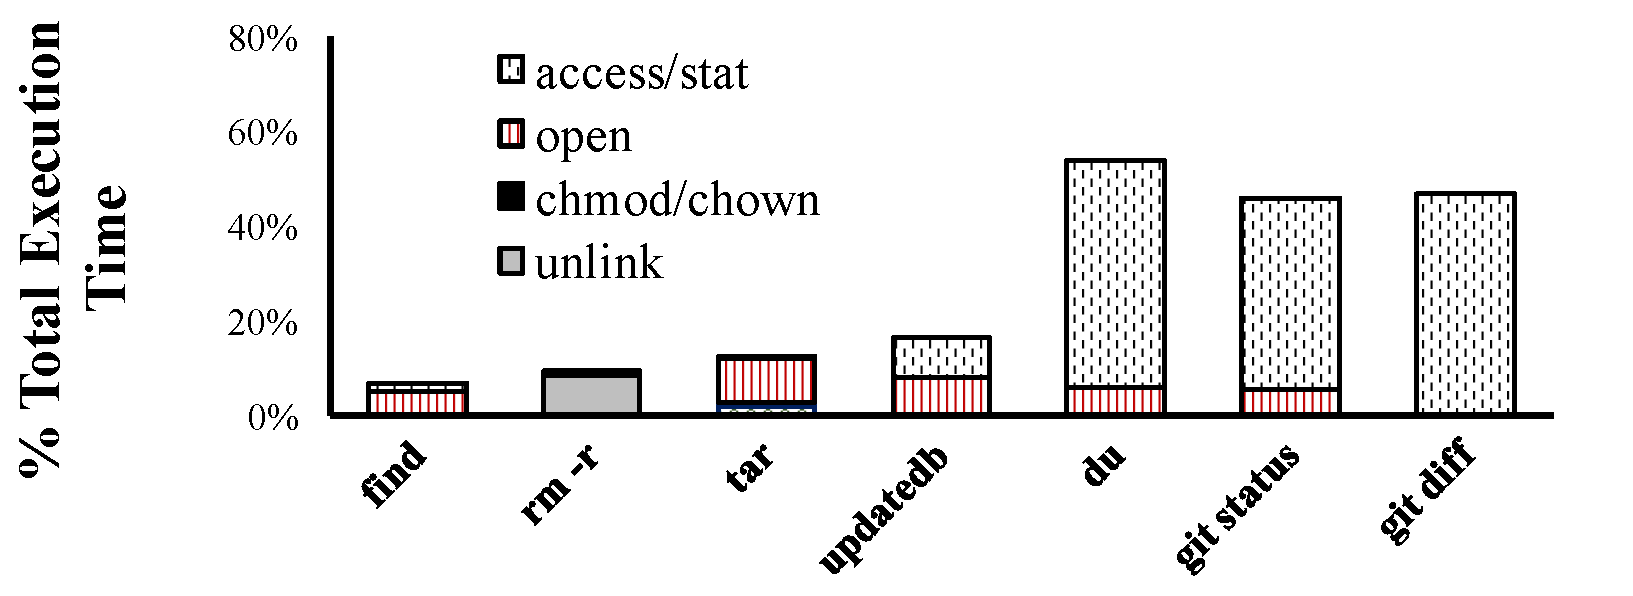
\includegraphics[width=5in]{dcache/plots/syscall-percentage.pdf} \\
\caption[Fraction of execution time on path-based system calls.]
{Fraction of execution time in several common utilities spent
executing path-based system calls with a warm cache, as measured with ftrace.}
\label{fig:dcache:lookup-frac}
%\vspace{-10pt}
\end{figure}

%\fixmedp{Please check these \% against time.  I think git diff is too high.  git status seems ok.}

Directory caches are essential for good application performance.
%Unix was designed such that ``(almost) everything is a file'',
%thus even accesses to in-memory file systems, device files, FIFOs and domain sockets
%first pass through the directory cache.
%In other words, 
Many common system calls must operate on file paths,
which require a directory cache lookup.
For instance, between 10--20\% of all system calls in the iBench system call traces do a path lookup~\citep{filenotafile}. 
Figure~\ref{fig:dcache:lookup-frac} lists the fraction of total execution time
%, as well as system time, 
several common command-line applications spend executing path-based system calls
(more details on these applications and the test machine in \S\ref{sec:dcache:eval}).
We note that these system calls include work other than path lookup,
and that these numbers include some instrumentation overhead;
% are coarse measurements that include  and work than path lookup;
%, and includes some time 
%for synchronous I/O (e.g., during {\tt rename}) as well as non-path tasks (e.g., creating 
%a file handle as part of {\tt open});
nonetheless, in all cases except {\tt rm},
the system call times and counts are dominated by
{\tt stat} and {\tt open}, for which 
%can be serviced from cache and for which 
path lookup is a significant component of execution time.
For these applications, path-based system calls account for 6--54\% of total execution time.
%and 25--77\% of system time.  
This implies that
lowering path lookup latency is
 one of the  biggest 
opportunities for a kernel to improve these applications' execution time.




\begin{figure}[t!]
\centering
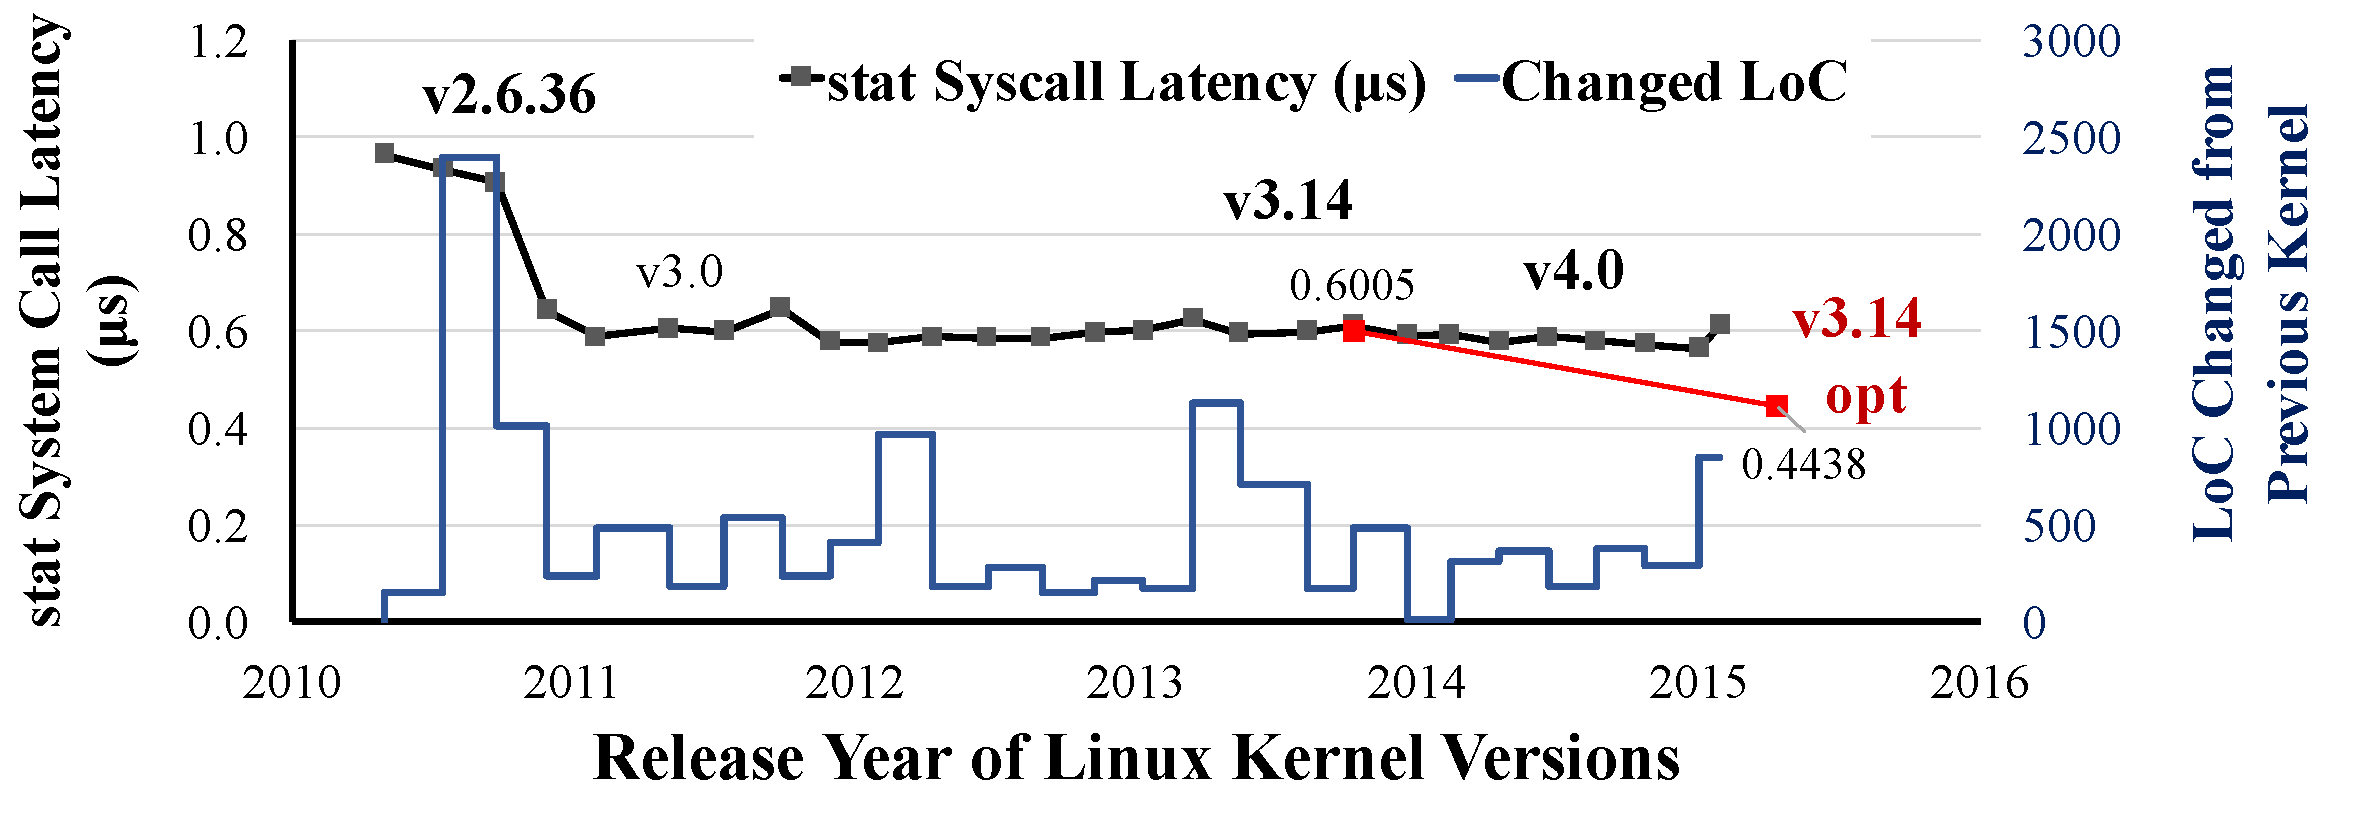
\includegraphics[width=6in]{dcache/plots/latency-by-version.pdf}
\footnotesize
\caption[Lantecy of {\tt stat} system call over years.]
{Latency of {\tt stat} system call with a long path {\tt XXX/YYY/ZZZ/AAA/BBB/CCC/DDD/FFF} on Linux over four years (lower is better), as well as the churn within the directory cache code (all insertions in {\tt dcache.c}, {\tt dcache.h}, {\tt namei.c}, {\tt namei.h} and {\tt namespace.c}). 
%Our optimizations significantly improve performance that has otherwise plateaued, despite significant ongoing developer effort.  
Our optimized \linuxver{} kernel 
further reduces {\tt stat} system call latency by \statspeedup{}\%.}
%\vspace{-15pt}
\label{fig:dcache:by-version}
\end{figure}


%\fixmedp{Add more evidence of lookup importance here: For instance, fraction of lookup time in file-related syscalls, or total lookup time in applications bound on file lookup latency.  }
Unfortunately, even directory cache hits are costly --- 0.3--1.1 \us{} for a {\tt stat} on our test Linux system, compared to only .04 \us{} for a {\tt getppid} and 0.3 \us{} for a 4 KB {\tt pread}. 
%\fixmetsai{Don, check this, I think read will be a better example, getppid is too trivial.}
This issue is taken particularly seriously in the Linux kernel community, which has 
made substantial revisions and increasingly elaborate optimizations to reduce the hit cost
of its directory cache, such as removing locks from the read path or replacing lock ordering with deadlock avoidance in a retry loop~\citep{corbet09jls,dcache-rcu}.
Figure~\ref{fig:dcache:by-version} plots directory cache hit latency against  lines of directory cache code changed 
over several versions of Linux, using a path-to-inode lookup \microbench{} on the test system described
in \S~\ref{sec:dcache:eval}.
These efforts have improved hit latency by 47\% from 2011 to 2013, but have plateaued
for the last three years.
%\fixmedp{if time, filter irrelevant changes from code deltas}
%at the cost of substantial developer effort.
%This latency appears to have plateaued 

The root of the problem is that the POSIX path permission semantics
seemingly require work that is linear in the number of path components,
and severely limit the kernel developer's implementation options.
%The root of this problem is that current directory cache
%designs reflect a straightforward implementation of the POSIX specification,
%which would seemingly require work that is linear in the number of path components.
For instance, in order to open file {\tt /\fnone{}/\fntwo{}/\fnthree{}} 
%for reading, 
one must have search permission
to parent directories {\tt /}, {\tt /\fnone{}}, and {\tt /\fnone{}/\fntwo{}},
as well as permission to access file {\tt \fnthree{}}.
The Linux implementation %of this specification is straightforward, 
simply walks the directory
tree top-down to check permissions.  
Unfortunately, when the critical path is dominated by 
walking a pointer-based data structure, 
including memory barriers on some architectures for multi-core consistency, 
modern CPUs end up stalling on hard-to-prefetch loads.
Moreover, because so many Linux features are built around this behavior, such as Linux Security Modules (LSMs)~\citep{wright+lsm},
namespaces, and mount aliases, it is not clear that any data-structural enhancements
are possible without breaking backward-compatibility with other Linux kernel features.
A priori, it is not obvious that a faster lookup algorithm, such as a single hash table lookup, 
can meet these API specifications and kernel-internal requirements; to our knowledge,
no one has tried previously.

%This paper proposes a decomposition of the directory cache, which allows
%most lookup operations to execute with a single hash table lookup (\S\ref{sec:dcache:dcache}),
%as well as optimizations to reduce the miss rate based on information that is {\em already in the cache}, but not used effectively (\S\ref{sec:dcache:readdir}).
%Our design maintains compatibility (\S\ref{sec:dcache:generalize}) through 
%several essential insights, including 
%how to separate the indexing of paths from checking parent permissions,
%and how to effectively and safely memoize the results of access control checks.


%% This paper proposes several new ways to organize a directory cache, which can yield 
%% substantial performance improvements over the current state of the art.
%% %This paper demonstrates that, despite this developer effort, there is still a substantial 
%% %missed opportunity hiding behind historical, intuitive, but not fundamental design choices.
%% Most of the Linux directory cache design reflects a straightforward implementation of the POSIX 
%% specification. %, with a division of labor that is suitable for mainstream file systems.

%This paper presents an alternative directory cache organization, which 
%improves performance by separating logical tasks, such as separating path indexing from permission checking; yet the design is sufficient to retain compatibility with POSIX.
%In the case of path lookup, 
%this paper demonstrates how 
%a per-component tree walk can be replaced with a single hash table lookup (\S\ref{sec:dcache:dcache}).
% without violating POSIX compliance.

%Our optimizations improve the performance of frequent lookup operations, but 
%introduce several costs, described in \S\ref{sec:dcache:dcache} and measured in \S\ref{sec:dcache:eval},
%which  we believe are acceptable and a net improvement for applications.
%First, these optimizations slow down infrequent modifications to the directory hierarchy, such as {\tt rename}, {\tt chmod},
% and {\tt chown} of a directory. 
%However, these slower operations
%account for less than .01\% of the system calls in the iBench traces~\citep{filenotafile}.
%Second,  the memory overheads of the dcache are increased.
%%(45\% per \dentry{}, as well as some  in our prototype).
%%(\fixmedp{XX MB} in our tests).  
%Third, lookup has a 
%probability of error from signature collisions that can be adjusted to be negligible
%%($2^{-141}$ in our configuration), 
%and within acceptable thresholds widely used by data deduplication systems~\citep{Debnath:2010:CSU:1855840.1855856, Srinivasan:2012:ILI:2208461.2208485, Quinlan:2002:VNA:645371.651321, Zhu:2008:ADB:1364813.1364831}.
%%, as well as how to remove
%%all memory barriers from the lookup path (\S\ref{sec:dcache:update}).
%In the micro-benchmark of Figure~\ref{fig:dcache:by-version}, our directory cache 
%optimizations improve lookup latency by 
%%revisions improve latency of accessing a long path
%%by 
%\statspeedup{}\% over unmodified Linux.
%%Our design addresses other missed
%%opportunities, such as identifying new opportunities to reduce the miss rate
%%through caching directory completeness.
%%\fixmedp{Do we want to highlight LoC?  3K is more than anything in the graph} \fixmetsai{Probably just mention in the evaluation. It's a metric that we should provide, but it's not awfully interesting.}
%%The total lines of code changed are fewer than 3,000 out of \fixmedp{XX}.
%%\fixmedp{Can we get 
%%, yet changes fewer than 3,000 lines of code.

%% SOSP cut - kind of long-winded
\begin{comment}
This paper rethinks current Linux directory cache design choices in light of the following goals:
\begin{compactitem}
\item {\bf Minimize the cost of a cache hit.} (\S\ref{sec:dcache:dcache}).
This means maximizing the benefit of temporal locality for frequent operations,
while pushing extra work of consistency maintenance onto less frequent, already-expensive operations.
%such as handling cache miss or updating massive metadata,
%in order to improve very frequent operations.
\item {\bf Maintain legacy compatibility.} (\S\ref{sec:dcache:generalize}).  Unix path semantics are complex, required by applications, file systems, and security modules, frustrating otherwise straightforward optimizations.  However tempting it may be to redesign path behavior to facilitate caching, path operations must exhibit the same behavior, with lower latency.
\item {\bf Never miss the same request twice in quick succession.} (\S\ref{sec:dcache:readdir}).  A number of less-frequent operations, such as reading a directory or secure temporary file creation, always miss in the cache {\em even if enough information is in cache to satisfy the operation.}  
%Of course, infrequent accesses should still be subject to a cache replacement policy, such as LRU.
\end{compactitem}
%Although directory caches must implement more complex semantics than a hardware memory cache,
%these principles should seem familiar to the reader with a basic architecture background.
%sadly, the Linux directory cache design violates all three.
\end{comment}

%This paper introduces several techniques to improve the performance of a directory cache,
%This paper explains several practical directory cache optimizations,
This paper demonstrates that these techniques improve performance for applications that use the directory cache heavily,
and the harm is minimal to applications that do not benefit.
%and that the worst case \microbench{} is only 12\% slower within \fixmedp{XX}\% of unmodified Linux.
%Each optimization we describe improves performance in isolation, and all can be combined.
%These optimizations change very few lines of code, and are backward-compatible with 
%legacy applications.  
%These changes are encapsulated in the VFS---individual file systems do not have to change their code.
%This paper describes a  prototype of these improvements implemented in Linux \linuxver{}.
%\S~\ref{sec:dcache:background} explains that the directory cache structure of Mac OS X, FreeBSD, and Solaris 
%are sufficiently similar that these principles should generalize.
%we compare and contrast Linux's directory cache
%with Mac OS X, FreeBSD, and Solaris in \S\ref{sec:dcache:background}, and explain inline how each
%optimization could be generalized to these other OS kernels.





%% \item {\bf Modularization and stackability}:
%% Any changes or optimizations must be implemented as modules inside Linux's VFS,
%% and can be stacked on top of the original design or any future optimizations. 
%% \item {\bf Backward compatibility}:
%% Any changes or optimizations must maintain least requirement of modifying any
%% file systems.
%% \item {\bf Generalization to other OSes}: Any changes or optimizations must be portable to other OSes with reasonable effort and change of design.




%% \dcache{} is proven to be effective on improving storage performance.
%% Experiments shows that,
%% in a Linux 3.x kernel, a \dcache{} with a xxx\% hit rate can speed up
%% metadata lookup and fetching time by xxx times.
%% \fixmetsai{experiment result, Linux version, and fs specs here}
%% However, we observed that Linux maintainers have made
%% constant and non-trivial efforts to improve \dcache{} in the Linux kernel.
%% We studied all \dcache{}-related source files in the Linux kernel Git repository,
%% and discovered that maintainers have committed
%% on average xxx revisions per source files.

%% We tested metadata lookup time on primary \dcache{}-related revisions.
%% Most changes on \dcache{} system only create xxx\%-xxx\% speed-up
%% than their predecessor.
%% \fixmetsai{result and graph here}.
%% Moreover, improvement to \dcache{} is still work-in-progress
%% for Linux maintainers.
%% \fixmetsai{reference to threads for latest dcache discussions}. 
%% All the evidences show that,
%% despite of significant reduction of storage operations,
%% efficiency of \dcache{} system internally still remains as a concern.

%% We argue that the design of \dcache{} needs to be carefully re-examined,
%% to fundamentally identify any missed opportunities that
%% improve value of \dcache{}.
%% At a high level, most optimization works for \dcache{} are focused on
%% improving ``how to cache'',
%% but we want to also lay eyes on ``what to cache'',
%% to ensure any valuable information returned from file systems
%% be captured by \dcache{} system.

%The contributions of this paper are as follows:
%\begin{compactitem}
%\item A performance analysis of the costs of path lookup and the opportunities
%to improve cache hit latency.
%\item A directory cache design that improves path lookup latency with a combination of techniques, including:
%  \begin{compactitem}
%  \item Indexing the directory cache by full path, reducing average-case lookup from linear to constant in the number of path components.
%  \item A Prefix Check Cache (PCC) that separates permission checking from path caching.  The PCC memoizes permission checks, and is compatible with LSMs~\citep{wright+lsm}.
%  \item Reducing the cost of checking for hash bucket collisions with path signatures.
%  \end{compactitem}
%\item Identifying opportunities to leverage metadata the kernel already has to reduce miss rates, such as tracking whether a directory is completely in cache.
%\item Carefully addressing numerous, subtle edge cases that would frustrate rote application of these techniques, such as integration with symbolic links and Linux namespaces.
%\item A thorough evaluation of these optimizations.  For instance, our optimizations improve throughput
%of the Dovecot IMAP server by up to \dovecotspeedup\% and latency of 
%updatedb by up to \updatedbspeedup{}\%.
%%git version control system by up to 25\%.
%
%\end{compactitem}
